% Capitolul 10: Recapitulare Comprehensivă
% Prezentare academică de calitate Harvard
% Program de licență, Academia de Studii Economice din București

\documentclass[9pt, aspectratio=169, t]{beamer}

% Asigură încadrarea conținutului pe diapozitive
\setbeamersize{text margin left=8mm, text margin right=8mm}

%=============================================================================
% CONFIGURARE TEMĂ ȘI STIL
%=============================================================================
\usetheme{default}
% Using default theme for clean header/footer control

% Color Palette (matching Redispatch PDF)
\definecolor{MainBlue}{RGB}{26, 58, 110}
\definecolor{AccentBlue}{RGB}{26, 58, 110}
\definecolor{IDAred}{RGB}{205, 0, 0}
\definecolor{DarkGray}{RGB}{51, 51, 51}
\definecolor{MediumGray}{RGB}{128, 128, 128}
\definecolor{LightGray}{RGB}{248, 248, 248}
\definecolor{VeryLightGray}{RGB}{235, 235, 235}
\definecolor{KeynoteGray}{RGB}{218, 218, 218}
\definecolor{SectionGray}{RGB}{120, 120, 120}
\definecolor{FooterGray}{RGB}{100, 100, 100}
\definecolor{Crimson}{RGB}{220, 53, 69}
\definecolor{Forest}{RGB}{46, 125, 50}
\definecolor{Amber}{RGB}{181, 133, 63}
\definecolor{Orange}{RGB}{230, 126, 34}
\definecolor{Purple}{RGB}{142, 68, 173}

% Gradient background (exact Keynote 315° gradient: white to RGB 218,218,218)
\setbeamertemplate{background}{%
    \begin{tikzpicture}[remember picture, overlay]
        \shade[shading=axis, shading angle=315,
        top color=white, bottom color=KeynoteGray]
        (current page.south west) rectangle (current page.north east);
    \end{tikzpicture}%
}
% Fallback solid color for compatibility
\setbeamercolor{background canvas}{bg=}

\setbeamercolor{palette primary}{bg=MainBlue, fg=white}
\setbeamercolor{palette secondary}{bg=MainBlue!85, fg=white}
\setbeamercolor{palette tertiary}{bg=MainBlue!70, fg=white}
\setbeamercolor{structure}{fg=MainBlue}
\setbeamercolor{title}{fg=IDAred}
\setbeamercolor{frametitle}{fg=IDAred, bg=}
\setbeamercolor{block title}{bg=MainBlue, fg=white}
\setbeamercolor{block body}{bg=VeryLightGray, fg=DarkGray}
\setbeamercolor{block title alerted}{bg=Crimson, fg=white}
\setbeamercolor{block body alerted}{bg=Crimson!8, fg=DarkGray}
\setbeamercolor{block title example}{bg=Forest, fg=white}
\setbeamercolor{block body example}{bg=Forest!8, fg=DarkGray}
\setbeamercolor{item}{fg=MainBlue}

% Footer colors (override Madrid theme blue)
\setbeamercolor{author in head/foot}{fg=FooterGray, bg=}
\setbeamercolor{title in head/foot}{fg=FooterGray, bg=}
\setbeamercolor{date in head/foot}{fg=FooterGray, bg=}
\setbeamercolor{section in head/foot}{fg=FooterGray, bg=}
\setbeamercolor{subsection in head/foot}{fg=FooterGray, bg=}

% Bullet styles (apply everywhere including blocks)
\setbeamertemplate{itemize item}{\color{MainBlue}$\boxdot$}
\setbeamertemplate{itemize subitem}{\color{MainBlue}$\blacktriangleright$}
\setbeamertemplate{itemize subsubitem}{\color{MainBlue}\tiny$\bullet$}
\setbeamertemplate{itemize/enumerate body begin}{\normalsize}
\setbeamertemplate{itemize/enumerate subbody begin}{\normalsize}

% Item spacing - compact style
\setlength{\leftmargini}{10pt}       % Level 1: minimal indent
\setlength{\leftmarginii}{10pt}      % Level 2: minimal additional indent
% Compact list spacing (zero extra space before/after lists in blocks)
\makeatletter
\def\@listi{\leftmargin\leftmargini \topsep 0pt \parsep 0pt \itemsep 0pt}
\def\@listii{\leftmargin\leftmarginii \topsep 0pt \parsep 0pt \itemsep 0pt}
\makeatother

\setbeamertemplate{navigation symbols}{}

%=============================================================================
% CUSTOM HEADLINE
%=============================================================================
\setbeamertemplate{headline}{%
    \vskip10pt%
    \hbox to \paperwidth{%
        \hskip0.5cm%
        {\small\color{FooterGray}\renewcommand{\hyperlink}[2]{##2}\insertsectionhead}%
        \hfill%
        \textcolor{FooterGray}{\small\insertframenumber}%
        \hskip0.5cm%
    }%
    \vskip4pt%
    {\color{FooterGray}\hrule height 0.4pt}%
}

%=============================================================================
% CUSTOM FOOTER
%=============================================================================
\usepackage{fontawesome5}

\setbeamertemplate{footline}{%
    {\color{FooterGray}\hrule height 0.4pt}%
    \vskip4pt%
    \hbox to \paperwidth{%
        \hskip0.5cm%
        \textcolor{FooterGray}{\small Analiza și Prognoza Seriilor de Timp}%
        \hfill%
        \raisebox{-0.1em}{%
            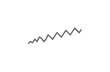
\begin{tikzpicture}[x=0.08em, y=0.08em, line width=0.4pt]
                \draw[FooterGray] (0,3) -- (1,4) -- (2,3.5) -- (3,5) -- (4,4) -- (5,6) -- (6,5.5) -- (7,4) -- (8,5) -- (9,7) -- (10,6) -- (11,5) -- (12,6.5) -- (13,8) -- (14,7) -- (15,6) -- (16,7.5) -- (17,9) -- (18,8) -- (19,7) -- (20,8.5) -- (21,10) -- (22,9) -- (23,8) -- (24,9.5);
            \end{tikzpicture}%
        }%
        \hskip0.5cm%
    }%
    \vskip6pt%
}

%=============================================================================
% PACHETE
%=============================================================================
\usepackage[utf8]{inputenc}
\usepackage[T1]{fontenc}
\usepackage{amsmath, amssymb, amsthm}
\usepackage{mathtools}
\usepackage{bm}
\usepackage{tikz}
\usetikzlibrary{arrows.meta, positioning, shapes, calc, decorations.pathreplacing, shadings}
\usepackage{booktabs}
\usepackage{multirow}
\usepackage{array}
\usepackage{graphicx}
\usepackage{hyperref}
\usepackage{colortbl}
\hypersetup{colorlinks=true, linkcolor=MainBlue, urlcolor=MainBlue}
\graphicspath{{../../logos/}{../../charts/}}
\hfuzz=2pt  % Suppress tiny overfull warnings (<2pt)
\vfuzz=2pt  % Suppress tiny vertical overfull warnings (<2pt)

%=============================================================================
% COMANDA QUANTLET
%=============================================================================
\newcommand{\quantlet}[2]{%
    \hfill\href{#2}{%
        \raisebox{-0.15em}{\includegraphics[height=0.7em]{ql_logo.png}}%
        \textcolor{MainBlue}{\tiny\ #1}%
    }%
}

%=============================================================================
% MEDII PENTRU TEOREME
%=============================================================================
\theoremstyle{definition}
\setbeamertemplate{theorems}[numbered]
\newtheorem{defn}{Definiție}
\newtheorem{thm}{Teoremă}
\newtheorem{prop}{Propoziție}
\newtheorem{rmk}{Observație}

%=============================================================================
% CENTRED MINIPAGE (fără spațiu vertical suplimentar)
%=============================================================================
\newenvironment{cminipage}[1]{%
    \par\noindent\hfill\begin{minipage}{#1}\ignorespaces
}{%
    \end{minipage}\hfill\null\par
}

%=============================================================================
% COMENZI PERSONALIZATE
%=============================================================================
\newcommand{\E}{\mathbb{E}}
\newcommand{\Var}{\text{Var}}
\newcommand{\Cov}{\text{Cov}}
\newcommand{\Corr}{\text{Corr}}
\newcommand{\R}{\mathbb{R}}
\newcommand{\N}{\mathbb{N}}
\newcommand{\Z}{\mathbb{Z}}
\newcommand{\B}{\mathbf{B}}
\newcommand{\imark}{\textcolor{MainBlue}{\textbullet}}
\newcommand{\RMSE}{\text{RMSE}}
\newcommand{\MAE}{\text{MAE}}
\newcommand{\MAPE}{\text{MAPE}}

%=============================================================================
% PAGINĂ TITLU PERSONALIZATĂ
%=============================================================================
\defbeamertemplate*{title page}{hybrid}[1][]
{
    \vspace{0.2cm}
    % Logos row - top header (with clickable links)
    \begin{center}
        \href{https://www.ase.ro}{\includegraphics[height=1.0cm]{ase_logo.png}}\hspace{0.3cm}%
        \href{https://theida.net}{\includegraphics[height=1.0cm]{ida_logo.png}}\hspace{0.3cm}%
        \href{https://blockchain-research-center.com}{\includegraphics[height=1.0cm]{brc_logo.png}}\hspace{0.3cm}%
        \href{https://www.ai4efin.ase.ro}{\includegraphics[height=1.0cm]{ai4efin_logo.png}}\hspace{0.3cm}%
        \href{https://ipe.ro/new}{\includegraphics[height=1.0cm]{acad_logo.png}}\hspace{0.3cm}%
        \href{https://www.digital-finance-msca.com}{\includegraphics[height=1.0cm]{msca_logo.png}}%
    \end{center}

    \vspace{0.6cm}

    % Main title with Q logos on sides (with clickable links)
    \begin{center}
        \begin{minipage}{0.1\textwidth}
            \centering
            \href{https://quantlet.com}{\includegraphics[height=1.1cm]{ql_logo.png}}
        \end{minipage}%
        \begin{minipage}{0.78\textwidth}
            \centering
            {\LARGE\bfseries\usebeamercolor[fg]{title}\inserttitle}

            \vspace{0.3cm}

            {\usebeamerfont{subtitle}\usebeamercolor[fg]{title}\insertsubtitle}
        \end{minipage}%
        \begin{minipage}{0.1\textwidth}
            \centering
            \href{https://quantinar.com}{\includegraphics[height=1.1cm]{qr_logo.png}}
        \end{minipage}
    \end{center}

    \vspace{0.6cm}

    % Authors (left aligned)
    \hspace{0.5cm}{\usebeamerfont{author}\insertauthor}

    \vspace{0.3cm}

    % Institute/Affiliations (left aligned)
    \hspace{0.5cm}\begin{minipage}[t]{0.9\textwidth}
        \raggedright\small\insertinstitute
    \end{minipage}
}

%=============================================================================
% INFORMAȚII TITLU
%=============================================================================
\title[Analiza Seriilor de Timp]{Analiza și Prognoza Seriilor de Timp}
\subtitle{Capitolul 10: Recapitulare Comprehensivă}
\author[D.T. Pele]{Daniel Traian PELE}
\institute{Academia de Studii Economice din București\\
IDA Institute Digital Assets\\
Blockchain Research Center\\
AI4EFin Artificial Intelligence for Energy Finance\\
Academia Română, Institutul de Prognoză Economică\\
MSCA Digital Finance}
\date{}

\begin{document}

% Title page (no header/footer)
{
\setbeamertemplate{headline}{}
\setbeamertemplate{footline}{}
\begin{frame}
    \titlepage
\end{frame}
}

%=============================================================================
% LEARNING OBJECTIVES
%=============================================================================
\begin{frame}{Obiective de învățare}
    \begin{cminipage}{0.95\textwidth}
    \begin{block}{La finalul acestui capitol, veți fi capabili să:}
        \begin{enumerate}\setlength{\itemsep}{0pt}
            \item Aplicați fluxul complet de prognoză, de la date la evaluare
            \item Selectați modelul potrivit în funcție de caracteristicile datelor
            \item Evaluați acuratețea prognozelor folosind metrici și validare încrucișată
            \item Integrați cunoștințele din toate capitolele anterioare în practică
        \end{enumerate}
    \end{block}
    \end{cminipage}
\end{frame}

%=============================================================================
% OUTLINE
%=============================================================================
\begin{frame}{Cuprins}
    \vspace{-0.2cm}
    {\small
    \begin{columns}[T]
        \begin{column}{0.48\textwidth}
            \begin{block}{Fundamente}
                \begin{itemize}\setlength{\itemsep}{3pt}
                    \item Metodologia Prognozei
                    \item Studiu de Caz 1: Volatilitatea Bitcoin (GARCH)
                    \item Studiu de Caz 2: Ciclurile Petelor Solare (Fourier)
                \end{itemize}
            \end{block}
        \end{column}
        \begin{column}{0.48\textwidth}
            \begin{exampleblock}{Aplicații}
                \begin{itemize}\setlength{\itemsep}{3pt}
                    \item Studiu de Caz 3: Șomajul (Prophet)
                    \item Studiu de Caz 4: Analiză Multivariată (VAR)
                    \item Sinteză și Ghid
                    \item Quiz
                \end{itemize}
            \end{exampleblock}
        \end{column}
    \end{columns}
    }
\end{frame}

%=============================================================================
% SECTION 1: METHODOLOGY
%=============================================================================
\section{Metodologia Prognozei}

\begin{frame}{Abordarea științifică a prognozei}
    \begin{cminipage}{0.95\textwidth}
    \begin{block}{Întrebarea de cercetare}
        \begin{itemize}\setlength{\itemsep}{0pt}
            \item Cum putem \textbf{evalua riguros} performanța prognozei evitând supraajustarea?
        \end{itemize}
    \end{block}

    \vspace{0.3cm}

    \begin{alertblock}{Problema fundamentală}
        \begin{itemize}
            \item Ajustarea în eșantion $\neq$ Performanța în afara eșantionului
            \item Modelele pot ``memora'' datele de antrenament fără a învăța tipare
            \item \textbf{Soluție}: Metodologia corectă train/validation/test
        \end{itemize}
    \end{alertblock}

    \vspace{0.3cm}

    \begin{exampleblock}{Principiu cheie}
        \begin{itemize}\setlength{\itemsep}{0pt}
            \item ``Setul de test trebuie să rămână \textbf{neatins} până la evaluarea finală.''
            \item Practică standard în machine learning și econometrie
        \end{itemize}
    \end{exampleblock}
    \end{cminipage}
\end{frame}

\begin{frame}{Cadrul Train/Validation/Test}
    \begin{center}
        \includegraphics[width=0.95\textwidth, height=0.78\textheight, keepaspectratio]{../charts/train_val_test_split.pdf}
    \end{center}
    \quantlet{TSA\_ch10\_train\_val\_test\_split}{https://github.com/QuantLet/TSA/tree/main/TSA_ch10/TSA_ch10_train_val_test_split}
\end{frame}

\begin{frame}{Metrici de evaluare}
    \begin{defn}[Metrici ale Erorii de Prognoză]
        \begin{itemize}\setlength{\itemsep}{0pt}
            \item \textbf{Date}: Fie $y_t$ valorile reale, $\hat{y}_t$ prognozele
        \end{itemize}
        \vspace{-0.2cm}
        \begin{align*}
            \RMSE = \sqrt{\frac{1}{n}\sum_{t}(y_t - \hat{y}_t)^2}, \quad
            \MAE = \frac{1}{n}\sum_{t}|y_t - \hat{y}_t|, \quad
            \MAPE = \frac{100\%}{n}\sum_{t}\left|\frac{y_t - \hat{y}_t}{y_t}\right|
        \end{align*}
    \end{defn}

    \begin{columns}[T]
        \column{0.5\textwidth}
        \begin{exampleblock}{Când să folosim}
            \begin{itemize}
                \item \textbf{RMSE}: Penalizează erorile mari
                \item \textbf{MAE}: Robust la outlieri
                \item \textbf{MAPE}: Independent de scală (\%)
            \end{itemize}
        \end{exampleblock}

        \column{0.5\textwidth}
        \begin{alertblock}{Atenție}
            \begin{itemize}
                \item MAPE nedefinit când $y_t = 0$
                \item Comparați pe \textbf{același} set test
                \item Raportați metrici \textbf{out-of-sample}
            \end{itemize}
        \end{alertblock}
    \end{columns}
\end{frame}

\begin{frame}{Evaluarea prognozelor dincolo de RMSE}
    \begin{columns}[T]
        \column{0.48\textwidth}
        \begin{block}{Metrici alternative}
            \begin{itemize}\setlength{\itemsep}{0pt}
                \item \textbf{MASE}: comparație cu naïve forecast
                \item \textbf{Directional Accuracy}: direcția corectă
                \item \textbf{Quantile Loss}: pentru VaR
                \item \textbf{CRPS}: distribuție completă
            \end{itemize}
        \end{block}

        \vspace{0.1cm}

        \begin{exampleblock}{Exemplu: Quantile Loss}
            \vspace{-0.2cm}
            \[
            QL_{\alpha} =
            \begin{cases}
            \alpha (y_t - \hat{q}_t), & y_t > \hat{q}_t \\
            (1-\alpha)(\hat{q}_t - y_t), & y_t \le \hat{q}_t
            \end{cases}
            \]
        \end{exampleblock}

        \column{0.50\textwidth}
        \begin{alertblock}{Rezultate Bitcoin (GARCH volatilitate)}
            \begin{tabular}{lc}
                \textbf{Metrică} & \textbf{Valoare} \\
                \midrule
                RMSE & 2.21 \\
                MAE & 1.89 \\
                MASE & 0.98 \\
                Dir. Accuracy & 28.7\% \\
            \end{tabular}
            \vspace{0.1cm}
            \begin{itemize}\setlength{\itemsep}{0pt}
                \item MASE $< 1$: GARCH bate naïve
                \item DA 28.7\%: direcția volatilității e dificilă
            \end{itemize}
        \end{alertblock}
    \end{columns}
\end{frame}

\begin{frame}{Compararea formală a prognozelor: Diebold--Mariano}
    \vspace{-0.2cm}
    \begin{defn}[Testul Diebold--Mariano]
        Diferența de pierdere: $d_t = L(e_{1t}) - L(e_{2t})$, \quad Statistica: $DM = \frac{\bar{d}}{\sqrt{\widehat{\text{Var}}(\bar{d})}} \xrightarrow{d} N(0,1)$
    \end{defn}

    \vspace{-0.1cm}

    \begin{columns}[T]
        \column{0.5\textwidth}
        \begin{block}{Ipoteze}
            \begin{itemize}\setlength{\itemsep}{0pt}
                \item $H_0$: performanță predictivă egală
                \item $H_1$: un model e semnificativ mai bun
                \item $|DM|$ mare $\Rightarrow$ respingem $H_0$
            \end{itemize}
        \end{block}

        \column{0.5\textwidth}
        \begin{exampleblock}{Rezultat Bitcoin (GARCH volatilitate)}
            \begin{itemize}\setlength{\itemsep}{0pt}
                \item Normal vs Student-t: $DM = -0.51$
                \item $p = 0.612$ --- \textbf{nu respingem} $H_0$
                \item Acuratețe similară, dar Student-t preferabil prin AIC ($\Delta = 509$)
            \end{itemize}
        \end{exampleblock}
    \end{columns}

    \vspace{0.1cm}

    \begin{alertblock}{Mesaj cheie}
        \begin{itemize}\setlength{\itemsep}{0pt}
            \item RMSE mai mic $\neq$ diferență semnificativă --- testarea formală este \textbf{obligatorie}
        \end{itemize}
    \end{alertblock}
\end{frame}

%=============================================================================
% SECTION 2: BITCOIN VOLATILITY
%=============================================================================
\section{Studiu de Caz 1: Volatilitatea Bitcoin (GARCH)}

\begin{frame}{Bitcoin: volatility clustering}
    \vspace{-0.2cm}
    {\scriptsize
    \begin{block}{Observație}
        \begin{itemize}\setlength{\itemsep}{0pt}
            \item Randamentele mari tind să urmeze randamente mari, cele mici urmează cele mici
            \item Acesta este \textbf{volatility clustering} $\succ$ fenomenul pe care GARCH îl captează
        \end{itemize}
    \end{block}
    }
    \begin{center}
        \includegraphics[width=0.95\textwidth, height=0.50\textheight, keepaspectratio]{../charts/btc_returns.pdf}
    \end{center}
    \quantlet{TSA\_ch10\_btc\_returns}{https://github.com/QuantLet/TSA/tree/main/TSA_ch10/TSA_ch10_btc_returns}
\end{frame}

\begin{frame}{Bitcoin: definirea problemei}
    \begin{block}{Întrebarea de cercetare}
        \begin{itemize}\setlength{\itemsep}{0pt}
            \item Putem prognoza \textbf{volatilitatea} Bitcoin folosind modele GARCH?
        \end{itemize}
    \end{block}

    \vspace{0.2cm}

    \begin{columns}[T]
        \column{0.5\textwidth}
        \textbf{Caracteristicile Datelor}
        \begin{itemize}
            \item Sursă: Yahoo Finance (BTC-USD)
            \item Perioadă: Ian 2019 -- Ian 2025
            \item Frecvență: Zilnică
            \item Observații: $\approx 2.200$ zile
        \end{itemize}

        \vspace{0.3cm}

        \textbf{Fapte stilizate}
        \begin{itemize}
            \item Randamente: medie aproape zero
            \item Cozi groase (curtosis $> 3$)
            \item Clustering al volatilității
        \end{itemize}

        \column{0.5\textwidth}
        \begin{alertblock}{Insight cheie}
            \begin{itemize}\setlength{\itemsep}{0pt}
                \item \textbf{Randamentele financiare} sunt de obicei:
                \begin{itemize}
                    \item Impredictibile în medie
                    \item Predictibile în varianță
                \end{itemize}
                \item $\succ$ Focus pe \textbf{prognoza volatilității}
            \end{itemize}
        \end{alertblock}
    \end{columns}
\end{frame}

\begin{frame}{Bitcoin: dovezi pentru GARCH}
    \vspace{-0.2cm}
    {\scriptsize
    }
    \begin{center}
        \includegraphics[width=0.95\textwidth, height=0.50\textheight, keepaspectratio]{../charts/btc_squared_returns.pdf}
    \end{center}
    \quantlet{TSA\_ch10\_btc\_acf\_squared}{https://github.com/QuantLet/TSA/tree/main/TSA_ch10/TSA_ch10_btc_acf_squared}
\end{frame}

\begin{frame}{Specificarea modelului GARCH}
    \vspace{-0.1cm}
    \begin{defn}[Modelul GARCH(p,q)]
        \begin{itemize}\setlength{\itemsep}{0pt}
            \item \textbf{Date}: Fie $r_t$ randamentele. Modelul GARCH(p,q) este:
        \end{itemize}
        \vspace{-0.2cm}
        \begin{align*}
            r_t &= \mu + \varepsilon_t, \quad \varepsilon_t = \sigma_t z_t, \quad z_t \sim N(0,1) \\[0.2cm]
            \sigma_t^2 &= \omega + \sum_{i=1}^{q}\alpha_i \varepsilon_{t-i}^2 + \sum_{j=1}^{p}\beta_j \sigma_{t-j}^2
        \end{align*}
        \vspace{-0.3cm}
        \begin{itemize}\setlength{\itemsep}{0pt}
            \item \textbf{Condiții}: $\omega > 0$, $\alpha_i \geq 0$, $\beta_j \geq 0$, și $\sum_{i=1}^{q}\alpha_i + \sum_{j=1}^{p}\beta_j < 1$
        \end{itemize}
    \end{defn}

    \vspace{0.1cm}

    {\small
    \begin{columns}[T]
        \column{0.5\textwidth}
        \begin{block}{Variante de model}
            \begin{itemize}\setlength{\itemsep}{0pt}
                \item \textbf{GARCH(1,1)}: Cel mai comun
                \item \textbf{GJR-GARCH}: Efect de levier
                \item \textbf{EGARCH}: Șocuri asimetrice
            \end{itemize}
        \end{block}

        \column{0.5\textwidth}
        \begin{block}{Interpretare}
            \begin{itemize}\setlength{\itemsep}{0pt}
                \item $\alpha$: Impactul șocurilor trecute
                \item $\beta$: Persistența volatilității
                \item $\alpha + \beta \approx 1$: Persistență înaltă
            \end{itemize}
        \end{block}
    \end{columns}
    }
\end{frame}

\begin{frame}{GARCH: Staționaritate și varianța necondiționată}
    \vspace{-0.2cm}
    \begin{thm}[Staționaritatea în Covarianță a GARCH(1,1)]
        Dacă $\alpha_1 + \beta_1 < 1$, atunci $\{\varepsilon_t\}$ este staționar în covarianță cu:
        \[
        \bar{\sigma}^2 = \E[\sigma_t^2] = \frac{\omega}{1 - \alpha_1 - \beta_1}
        \]
    \end{thm}

    \vspace{-0.1cm}

    {\small
    \begin{exampleblock}{Derivare}
        Luăm speranța ambelor părți ale ecuației varianței:
        \begin{align*}
            \E[\sigma_t^2] &= \omega + \alpha_1 \E[\varepsilon_{t-1}^2] + \beta_1 \E[\sigma_{t-1}^2] \\
            \bar{\sigma}^2 &= \omega + (\alpha_1 + \beta_1)\bar{\sigma}^2 \quad \text{(staționaritate)} \\
            \bar{\sigma}^2 &= \frac{\omega}{1 - \alpha_1 - \beta_1}
        \end{align*}
    \end{exampleblock}
    }

    \vspace{0.0cm}

    \begin{alertblock}{Prognozele multi-step converg la $\bar{\sigma}^2$}
        Când $h \to \infty$: $\E_t[\sigma_{t+h}^2] \to \bar{\sigma}^2$ cu rata $(\alpha_1 + \beta_1)^h$.
    \end{alertblock}
\end{frame}

\begin{frame}{Bitcoin: selectarea modelului pe setul de validare}
    \vspace{-0.2cm}
    {\scriptsize
    \begin{block}{Metodologie}
            \begin{itemize}\setlength{\itemsep}{0pt}
                \item Estimăm fiecare model pe \textbf{datele de antrenament}, evaluăm pe \textbf{setul de validare}
            \end{itemize}
        \end{block}

        \vspace{0.0cm}

        \begin{center}
        \begin{tabular}{lcccl}
            \toprule
            \textbf{Model} & \textbf{AIC} & \textbf{BIC} & \textbf{Val MAE} & \textbf{Selectare} \\
            \midrule
            GARCH(1,1) & 6.994,8 & 7.020,6 & \textbf{2,638} & \cellcolor{Forest!20}\textbf{Cel mai bun} \\
            GARCH(2,1) & 6.993,7 & 7.024,6 & 2,640 & \\
            GJR-GARCH(1,1) & 6.983,7 & 7.014,6 & 2,669 & \\
            EGARCH(1,1) & --- & --- & --- & Eșuat$^*$ \\
            \bottomrule
        \end{tabular}
        \end{center}

        \vspace{0.0cm}
        {\footnotesize $^*$Prognoze analitice indisponibile pentru $h > 1$}

        \vspace{0.05cm}

        \begin{exampleblock}{Rezultat}
            \begin{itemize}\setlength{\itemsep}{0pt}
                \item \textbf{GARCH(1,1)} selectat pe baza celui mai mic MAE de validare pentru prognozele de volatilitate
            \end{itemize}
        \end{exampleblock}
    }
    \vspace{-0.25cm}
    \begin{center}
        \includegraphics[width=0.95\textwidth, height=0.18\textheight, keepaspectratio]{../charts/garch_forecast.pdf}
    \end{center}
    \quantlet{TSA\_ch10\_garch\_forecast}{https://github.com/QuantLet/TSA/tree/main/TSA_ch10/TSA_ch10_garch_forecast}
\end{frame}

\begin{frame}{Bitcoin: împărțirea datelor și staționaritate}
    \vspace{-0.1cm}
    \begin{columns}[T]
        \column{0.5\textwidth}
        \begin{block}{Împărțirea datelor}
            \begin{center}
            \begin{tabular}{lrr}
                \toprule
                \textbf{Set} & \textbf{Perioadă} & \textbf{N} \\
                \midrule
                Antrenament (70\%) & 2019-01 -- 2023-03 & 1.543 \\
                Validare (20\%) & 2023-03 -- 2024-06 & 441 \\
                Test (10\%) & 2024-06 -- 2025-01 & 221 \\
                \midrule
                \textbf{Total} & & \textbf{2.205} \\
                \bottomrule
            \end{tabular}
            \end{center}
        \end{block}

        \column{0.5\textwidth}
        \begin{block}{Teste de staționaritate}
            \begin{center}
            \begin{tabular}{lcc}
                \toprule
                \textbf{Serie} & \textbf{ADF} & \textbf{Rezultat} \\
                \midrule
                Prețuri & $p = 0.50$ & Non-staționară \\
                Randamente & $p < 0.01$ & \textcolor{Forest}{Staționară} \\
                \bottomrule
            \end{tabular}
            \end{center}

            \vspace{0.1cm}

            $\succ$ Modelăm \textbf{randamente}, nu prețuri
        \end{block}
    \end{columns}

    \vspace{0.2cm}

    \begin{alertblock}{De ce contează staționaritatea}
        \begin{itemize}\setlength{\itemsep}{0pt}
            \item \textbf{GARCH}: necesită input slab staționar
            \item \textbf{Prețuri vs Randamente}: Prețurile urmează random walk, randamentele sunt staționare
        \end{itemize}
    \end{alertblock}
\end{frame}

\begin{frame}{GARCH: prognozele multi-step converg}
    \vspace{-0.2cm}
    {\scriptsize
    \begin{exampleblock}{Insight cheie}
        \begin{itemize}\setlength{\itemsep}{0pt}
            \item Prognozele multi-step converg la $\bar{\sigma}^2 = \frac{\omega}{1-\alpha-\beta}$
            \item Soluția: prognoze rolling one-step-ahead
        \end{itemize}
    \end{exampleblock}
    }
    \begin{center}
        \includegraphics[width=0.95\textwidth, height=0.50\textheight, keepaspectratio]{../charts/garch_convergence.pdf}
    \end{center}
    \quantlet{TSA\_ch10\_garch\_convergence}{https://github.com/QuantLet/TSA/tree/main/TSA_ch10/TSA_ch10_garch_convergence}
\end{frame}

\begin{frame}{GARCH: soluția rolling one-step-ahead}
    \begin{center}
        \includegraphics[width=0.95\textwidth, height=0.78\textheight, keepaspectratio]{../charts/rolling_vs_multistep.pdf}
    \end{center}
    \quantlet{TSA\_ch10\_rolling\_vs\_multistep}{https://github.com/QuantLet/TSA/tree/main/TSA_ch10/TSA_ch10_rolling_vs_multistep}
\end{frame}

\begin{frame}{Bitcoin: Fapte stilizate GARCH}
    \begin{center}
        \includegraphics[width=0.95\textwidth, height=0.78\textheight, keepaspectratio]{../charts/btc_squared_returns.pdf}
    \end{center}
\end{frame}

\begin{frame}{GARCH: Distribuții pentru inovații}
    \vspace{-0.2cm}
    \begin{block}{Model}
        \vspace{-0.2cm}
        \[
        r_t = \mu + \sigma_t z_t
        \]
        \begin{itemize}\setlength{\itemsep}{0pt}
            \item Variante pentru $z_t$: $\mathcal{N}(0,1)$ (normală) sau $t_{\nu}$ (cozi groase)
        \end{itemize}
    \end{block}

    \vspace{-0.1cm}

    \begin{columns}[T]
        \column{0.5\textwidth}
        \begin{alertblock}{Bitcoin: dovezi empirice}
            \begin{itemize}\setlength{\itemsep}{0pt}
                \item Kurtosis reziduuri: \textbf{13.81} (Normal = 3)
                \item Skewness: $-0.29$
                \item Jarque-Bera: $9085$, $p < 0.001$
                \item Normalitatea \textbf{subestimează} riscul extrem
            \end{itemize}
        \end{alertblock}

        \column{0.5\textwidth}
        \begin{exampleblock}{Student-t: alegerea corectă}
            \begin{itemize}\setlength{\itemsep}{0pt}
                \item $\hat{\nu} = 2.96$ grade de libertate
                \item AIC Normal: 9769 vs Student-t: \textbf{9260}
                \item $\Delta$AIC = 509 --- dovadă \textbf{copleșitoare}
                \item Cozi groase = estimări VaR \textbf{mai realiste}
            \end{itemize}
        \end{exampleblock}
    \end{columns}
\end{frame}

\begin{frame}{Aplicație: Value-at-Risk condiționat}
    \vspace{-0.2cm}
    \begin{columns}[T]
    \begin{column}{0.45\textwidth}
    {\footnotesize
    \begin{defn}[VaR condiționat la nivel $\alpha$]
        \vspace{-0.2cm}
        \[
        \text{VaR}_{t+1}^{\alpha} = \mu_{t+1} + \sigma_{t+1} \cdot z_{\alpha}
        \]
    \end{defn}
    \vspace{-0.2cm}
    \begin{exampleblock}{Rezultate Bitcoin (test: 329 zile)}
        \begin{tabular}{lcc}
            & \textbf{Normal} & \textbf{Student-t} \\
            \midrule
            Încălcări 5\% & 12 (3.6\%) & \textbf{17 (5.2\%)} \\
            Încălcări 1\% & 1 (0.3\%) & 0 (0.0\%) \\
            Kupiec $p$ (5\%) & 0.238 & \textbf{0.890} \\
        \end{tabular}
    \end{exampleblock}
    \vspace{-0.1cm}
    {\scriptsize Student-t: 5.2\% $\approx$ 5\% --- acoperire perfectă. Normal: prea conservator (3.6\%).}
    }
    \end{column}
    \begin{column}{0.53\textwidth}
        \includegraphics[width=\textwidth, height=0.65\textheight, keepaspectratio]{ch10_btc_var_backtest.pdf}
    \end{column}
    \end{columns}
    \quantlet{TSA\_ch10\_empirical\_slides}{https://github.com/QuantLet/TSA/tree/main/TSA_ch10/TSA_ch10_empirical_slides}
\end{frame}

\begin{frame}{Validarea modelului de risc: Backtesting}
    \vspace{-0.2cm}
    {\footnotesize
    \begin{columns}[T]
        \column{0.48\textwidth}
        \begin{block}{Kupiec Test (Unconditional Coverage)}
            \vspace{-0.2cm}
            \[
            LR_{uc} = -2 \ln \left(
            \frac{(1-\alpha)^{T-x} \alpha^x}
            {(1-\hat{p})^{T-x} \hat{p}^x}
            \right) \sim \chi^2(1)
            \]
        \end{block}
        \vspace{-0.15cm}
        \begin{block}{Christoffersen (Independență)}
            \begin{itemize}\setlength{\itemsep}{0pt}
                \item Verifică \textbf{independența} încălcărilor
                \item $LR_{cc} = LR_{uc} + LR_{ind} \sim \chi^2(2)$
            \end{itemize}
        \end{block}

        \column{0.50\textwidth}
        \begin{exampleblock}{Rezultate Bitcoin (VaR 5\%)}
            \begin{tabular}{lcc}
                & \textbf{Normal} & \textbf{Student-t} \\
                \midrule
                Încălcări & 12/329 & 17/329 \\
                Rata & 3.6\% & \textbf{5.2\%} \\
                Kupiec $LR$ & 1.39 & \textbf{0.02} \\
                Kupiec $p$ & 0.238 & \textbf{0.890} \\
                Chr. $LR_{ind}$ & 0.00 & 1.20 \\
                Chr. $p$ & 1.000 & 0.272 \\
            \end{tabular}
        \end{exampleblock}
        \vspace{-0.15cm}
        \begin{alertblock}{Concluzie}
            \begin{itemize}\setlength{\itemsep}{0pt}
                \item Ambele trec Kupiec ($p > 0.05$)
                \item Student-t: acoperire \textbf{mai precisă}
            \end{itemize}
        \end{alertblock}
    \end{columns}
    }
\end{frame}

\begin{frame}{Limitările GARCH și extensii moderne}
    \begin{columns}[T]
        \column{0.5\textwidth}
        \begin{alertblock}{Limitări}
            \begin{itemize}\setlength{\itemsep}{0pt}
                \item Nu captează \textbf{jump-uri} (salturi bruște)
                \item Parametri constanți în timp
                \item Sensibil la distribuția aleasă
                \item Nu modelează \textbf{regimuri} diferite
            \end{itemize}
        \end{alertblock}

        \column{0.5\textwidth}
        \begin{exampleblock}{Extensii}
            \begin{itemize}\setlength{\itemsep}{0pt}
                \item \textbf{GJR-GARCH}: efect de levier
                \item \textbf{EGARCH}: șocuri asimetrice
                \item \textbf{Markov-Switching GARCH}: regimuri
                \item Volatilitate realizată (HAR)
                \item Hybrid GARCH + ML
            \end{itemize}
        \end{exampleblock}
    \end{columns}

    \vspace{0.3cm}

    \begin{block}{Mesaj cheie}
        \begin{itemize}\setlength{\itemsep}{0pt}
            \item GARCH este un \textbf{punct de plecare}, nu finalul modelării riscului
        \end{itemize}
    \end{block}
\end{frame}

\begin{frame}{Bitcoin: Concluzii cheie}
    \begin{columns}[T]
        \column{0.6\textwidth}
        \begin{block}{Sumar}
            \begin{enumerate}
                \item \textbf{Randamentele sunt staționare}; prețurile nu
                \item \textbf{GARCH(1,1)} depășește variantele mai complexe
                \item \textbf{Persistență înaltă} ($\alpha + \beta = 0,93$)
                \item Volatilitatea este \textbf{predictibilă} chiar când randamentele nu sunt
            \end{enumerate}
        \end{block}

        \vspace{0.3cm}

        \begin{exampleblock}{Implicații practice}
            \begin{itemize}
                \item Managementul riscului: VaR, Expected Shortfall
                \item Evaluarea opțiunilor necesită prognoze de volatilitate
                \item Optimizarea portofoliului cu risc variabil în timp
            \end{itemize}
        \end{exampleblock}

        \column{0.4\textwidth}
        \begin{alertblock}{Limitări}
            \begin{itemize}
                \item GARCH presupune șocuri \textbf{simetrice}
                \item Nu captează \textbf{salturi}
                \item Distribuția normală poate fi restrictivă
            \end{itemize}
        \end{alertblock}

        \vspace{0.3cm}

        \begin{block}{Extensii}
            \begin{itemize}
                \item Inovații Student-t
                \item Volatilitate realizată
                \item Modele HAR
            \end{itemize}
        \end{block}
    \end{columns}
\end{frame}

%=============================================================================
% SECTION 3: SUNSPOTS
%=============================================================================
\section{Studiu de Caz 2: Ciclurile Petelor Solare (Fourier)}

\begin{frame}{Pete solare: ciclul solar de 11 ani}
    \vspace{-0.2cm}
    {\scriptsize
    }
    \begin{center}
        \includegraphics[width=0.95\textwidth, height=0.50\textheight, keepaspectratio]{../charts/sunspots.pdf}
    \end{center}
    \quantlet{TSA\_ch10\_sunspots\_acf}{https://github.com/QuantLet/TSA/tree/main/TSA_ch10/TSA_ch10_sunspots_acf}
\end{frame}

\begin{frame}{Termeni Fourier pentru sezonalitate}
    \begin{center}
        \includegraphics[width=0.95\textwidth, height=0.78\textheight, keepaspectratio]{../charts/fourier_terms.pdf}
    \end{center}
    \quantlet{TSA\_ch10\_fourier\_terms}{https://github.com/QuantLet/TSA/tree/main/TSA_ch10/TSA_ch10_fourier_terms}
\end{frame}

\begin{frame}{Pete solare: selectarea modelului}
    \vspace{-0.1cm}
    \begin{block}{Metodologie}
        \begin{itemize}\setlength{\itemsep}{0pt}
            \item \textbf{Comparație}: $K = 1, 2, 3, 4$ armonici Fourier pe setul de validare
        \end{itemize}
    \end{block}

    \vspace{0.1cm}

    \begin{columns}[T]
        \column{0.5\textwidth}
        \begin{center}
        \textbf{Împărțirea Datelor}
        \begin{tabular}{lrr}
            \toprule
            \textbf{Set} & \textbf{Perioadă} & \textbf{N} \\
            \midrule
            Antrenament (70\%) & 1900--1975 & 76 \\
            Validare (20\%) & 1976--1997 & 22 \\
            Test (10\%) & 1998--2008 & 11 \\
            \midrule
            \textbf{Total} & & \textbf{109} \\
            \bottomrule
        \end{tabular}
        \end{center}

        \column{0.5\textwidth}
        \begin{center}
        \textbf{Comparație Modele}
        \begin{tabular}{cccc}
            \toprule
            \textbf{K} & \textbf{AIC} & \textbf{Val RMSE} & \\
            \midrule
            1 & 665,9 & 87,15 & \\
            2 & 668,0 & 86,92 & \\
            \rowcolor{Forest!20} 3 & 671,8 & \textbf{86,81} & Cel mai bun \\
            4 & 674,5 & 87,93 & \\
            \bottomrule
        \end{tabular}
        \end{center}
    \end{columns}

    \vspace{0.1cm}

    \begin{exampleblock}{Rezultat}
        \begin{itemize}\setlength{\itemsep}{0pt}
            \item \textbf{K = 3} armonici Fourier selectate (6 parametri pentru ciclul de 11 ani)
        \end{itemize}
    \end{exampleblock}
\end{frame}

\begin{frame}{Overfitting în alegerea lui $K$}
    \begin{columns}[T]
        \column{0.5\textwidth}
        \begin{alertblock}{Riscul de overfitting}
            \begin{itemize}\setlength{\itemsep}{0pt}
                \item $K$ prea mare $=$ memorare ciclu istoric
                \item Modelul se potrivește pe zgomot, nu pe semnal
                \item Performanța pe test se \textbf{degradează}
            \end{itemize}
        \end{alertblock}

        \vspace{0.2cm}

        \begin{block}{Fourier $\approx$ regresie periodică}
            \begin{itemize}\setlength{\itemsep}{0pt}
                \item Fiecare armonic adaugă 2 parametri ($\sin$, $\cos$)
                \item $K = 3$: 6 parametri suplimentari
                \item $K = 6$: 12 parametri --- risc supraajustare
            \end{itemize}
        \end{block}

        \column{0.5\textwidth}
        \begin{exampleblock}{Soluția: validare}
            \begin{itemize}\setlength{\itemsep}{0pt}
                \item Selectăm $K$ pe setul de \textbf{validare}
                \item Evaluăm pe \textbf{test} --- neatins
                \item Trade-off: complexitate vs generalizare
            \end{itemize}
        \end{exampleblock}

        \vspace{0.2cm}

        \begin{block}{La noi}
            \begin{itemize}\setlength{\itemsep}{0pt}
                \item $K = 3$ minimizează Val RMSE
                \item $K = 4$ crește eroarea $\succ$ overfitting
            \end{itemize}
        \end{block}
    \end{columns}
\end{frame}

\begin{frame}{Pete solare: rezultate prognoză}
    \begin{center}
        \includegraphics[width=0.95\textwidth, height=0.78\textheight, keepaspectratio]{../charts/sunspot_forecast.pdf}
    \end{center}
    \quantlet{TSA\_ch10\_sunspot\_forecast}{https://github.com/QuantLet/TSA/tree/main/TSA_ch10/TSA_ch10_sunspot_forecast}
\end{frame}

\begin{frame}{Pete solare: concluzii cheie}
    \begin{columns}[T]
        \column{0.5\textwidth}
        \begin{block}{Când să folosiți termeni Fourier}
            \begin{itemize}
                \item Perioada sezonieră $s$ este \textbf{lungă} (ex: 11 ani, 52 săptămâni)
                \item SARIMA ar necesita prea multe lag-uri sezoniere
                \item Tiparul este \textbf{neted și periodic}
                \item Trebuie capturate cicluri multiple
            \end{itemize}
        \end{block}

        \vspace{0.2cm}

        \begin{alertblock}{Alegerea lui K}
            \begin{itemize}\setlength{\itemsep}{0pt}
                \item \textbf{Strategie}: Începeți cu $K=1$, creșteți progresiv
                \begin{itemize}
                    \item Opriți când eroarea de validare nu mai scade
                    \item $K$ prea mare = supraajustare
                \end{itemize}
            \end{itemize}
        \end{alertblock}

        \column{0.5\textwidth}
        \begin{exampleblock}{Fourier vs SARIMA}
            \begin{center}
            \begin{tabular}{lcc}
                \toprule
                & \textbf{Fourier} & \textbf{SARIMA} \\
                \midrule
                Sezoane lungi & \checkmark & $\times$ \\
                Sezoane scurte & OK & \checkmark \\
                Parametri & $2K$ & Mulți \\
                Flexibilitate & Fixă & Adaptivă \\
                \bottomrule
            \end{tabular}
            \end{center}
        \end{exampleblock}

        \vspace{0.2cm}

        \begin{block}{Aplicații}
            \begin{itemize}\setlength{\itemsep}{0pt}
                \item \textbf{Domenii}: Cicluri climatice, cicluri de afaceri, fenomene astronomice
            \end{itemize}
        \end{block}
    \end{columns}
\end{frame}

%=============================================================================
% SECTION 4: UNEMPLOYMENT
%=============================================================================
\section{Studiu de Caz 3: Șomajul (Prophet)}

\begin{frame}{Șomajul: Train / Validation / Test Split}
    \vspace{-0.2cm}
    {\footnotesize
    \begin{block}{Metodologie}
            \begin{itemize}\setlength{\itemsep}{0pt}
                \item \textbf{Training} (70\%): Estimare modele
                \item \textbf{Validare} (20\%): Selecție model
                \item \textbf{Test} (10\%): Evaluare finală
            \end{itemize}
        \end{block}
    }
    \begin{center}
        \includegraphics[width=0.95\textwidth, height=0.50\textheight, keepaspectratio]{../charts/unemployment_train_val_test.pdf}
    \end{center}
    \quantlet{TSA\_ch10\_unemployment\_train\_val\_test}{https://github.com/QuantLet/TSA/tree/main/TSA_ch10/TSA_ch10_unemployment_train_val_test}
\end{frame}

\begin{frame}{Șomajul: analiză preliminară}
    \begin{center}
        \includegraphics[width=0.95\textwidth, height=0.78\textheight, keepaspectratio]{../charts/unemployment_acf_pacf.pdf}
    \end{center}
    \quantlet{TSA\_ch10\_unemployment\_acf\_pacf}{https://github.com/QuantLet/TSA/tree/main/TSA_ch10/TSA_ch10_unemployment_acf_pacf}
\end{frame}

\begin{frame}{Șomajul: teste de staționaritate}
    \begin{center}
        \includegraphics[width=0.95\textwidth, height=0.78\textheight, keepaspectratio]{../charts/unemployment_stationarity.pdf}
    \end{center}
    \quantlet{TSA\_ch10\_unemployment\_stationarity}{https://github.com/QuantLet/TSA/tree/main/TSA_ch10/TSA_ch10_unemployment_stationarity}
\end{frame}

\begin{frame}{Rupturi structurale: abordare formală}
    \begin{columns}[T]
        \column{0.5\textwidth}
        \begin{block}{Metode clasice}
            \begin{itemize}\setlength{\itemsep}{0pt}
                \item \textbf{Chow Test}: ruptură la punct cunoscut
                \item \textbf{Bai--Perron}: rupturi multiple, necunoscute
                \item \textbf{CUSUM}: detectare secvențială
            \end{itemize}
        \end{block}

        \vspace{0.1cm}

        \begin{alertblock}{Problemă}
            \begin{itemize}\setlength{\itemsep}{0pt}
                \item ADF poate confunda \textbf{break} cu \textbf{unit root}
                \item Test Zivot--Andrews: ADF cu ruptură endogenă
            \end{itemize}
        \end{alertblock}

        \column{0.5\textwidth}
        \begin{exampleblock}{Rezultat: Șomaj la COVID (martie 2020)}
            \begin{itemize}\setlength{\itemsep}{0pt}
                \item Chow Test: $F = 21.73$, $p < 0.001$
                \item Ruptură structurală \textbf{confirmată}
                \item SARIMA: parametri constanți --- risc
                \item Prophet: detectează changepoints automat
            \end{itemize}
        \end{exampleblock}

        \vspace{0.1cm}

        \begin{block}{Mesaj cheie}
            \begin{itemize}\setlength{\itemsep}{0pt}
                \item Modelul trebuie adaptat la \textbf{stabilitatea parametrilor}
            \end{itemize}
        \end{block}
    \end{columns}
\end{frame}

\begin{frame}{Șomajul: selecția modelului (set validare)}
    \vspace{-0.2cm}
    {\scriptsize
    \begin{block}{Best: SARIMA(1,1,1)(1,0,0)$_{12}$}
        \begin{itemize}\setlength{\itemsep}{0pt}
            \item Fit pe training (70\%), evaluare pe validare (20\%)
            \item Cel mai bun model selectat după Val RMSE minim
        \end{itemize}
    \end{block}
    }
    \begin{center}
        \includegraphics[width=0.95\textwidth, height=0.50\textheight, keepaspectratio]{../charts/sarima_model_selection.pdf}
    \end{center}
    \quantlet{TSA\_ch10\_sarima\_model\_selection}{https://github.com/QuantLet/TSA/tree/main/TSA_ch10/TSA_ch10_sarima_model_selection}
\end{frame}

\begin{frame}{Șomajul: parametrii SARIMA}
    \vspace{-0.2cm}
    {\footnotesize
    \begin{block}{SARIMA(1,1,1)(1,0,0)$_{12}$ estimat pe Train+Val (2010-2019)}
            \begin{itemize}\setlength{\itemsep}{0pt}
                \item AR(1): $\phi_1 = -0,86$
                \item MA(1): $\theta_1 = 0,78$
                \item SAR(12): $\Phi_1 = -0,08$ (n.s.)
            \end{itemize}
        \end{block}
    }
    \begin{center}
        \includegraphics[width=0.95\textwidth, height=0.50\textheight, keepaspectratio]{../charts/sarima_parameters.pdf}
    \end{center}
    \quantlet{TSA\_ch10\_sarima\_parameters}{https://github.com/QuantLet/TSA/tree/main/TSA_ch10/TSA_ch10_sarima_parameters}
\end{frame}

\begin{frame}{Testul Ljung-Box pentru autocorelația reziduurilor}
    \vspace{-0.2cm}
    {\scriptsize
    \begin{defn}[Testul Ljung-Box]
            Pentru reziduurile $\hat{\varepsilon}_t$ cu autocorelații eșantion $\hat{\rho}_k$, statistica de test:
            \[
            Q(h) = n(n+2) \sum_{k=1}^{h} \frac{\hat{\rho}_k^2}{n-k} \stackrel{H_0}{\sim} \chi^2(h-p-q)
            \]
            unde $p, q$ sunt ordinele ARMA. $H_0$: Reziduurile sunt zgomot alb.
        \end{defn}

        \begin{block}{Interpretare}
            \begin{itemize}
                \item $Q$ mare (p-value mic): Respingem $H_0$, reziduurile au structură
                \item $Q$ mic (p-value mare): Nu respingem $H_0$, modelul este adecvat
                \item Regulă practică: Folosiți $h = \min(10, n/5)$ pentru ordinul lag-ului
            \end{itemize}
        \end{block}
    }
    \begin{center}
        \includegraphics[width=0.95\textwidth, height=0.18\textheight, keepaspectratio]{../charts/sarima_diagnostics.pdf}
    \end{center}
\end{frame}

\begin{frame}{Șomajul: Diagnosticare SARIMA}
    \begin{center}
        \includegraphics[width=0.95\textwidth, height=0.78\textheight, keepaspectratio]{../charts/sarima_diagnostics.pdf}
    \end{center}
    \quantlet{TSA\_ch10\_sarima\_diagnostics}{https://github.com/QuantLet/TSA/tree/main/TSA_ch10/TSA_ch10_sarima_diagnostics}
\end{frame}

\begin{frame}{Șomajul: prognoza rolling SARIMA}
    \vspace{-0.2cm}
    {\scriptsize
    \begin{alertblock}{Problemă: Ruptura structurală}
        \begin{itemize}\setlength{\itemsep}{0pt}
            \item Prognoză rolling one-step-ahead (re-estimare la fiecare $t$)
            \item \textbf{Test RMSE = 0,12}
        \end{itemize}
    \end{alertblock}
    }
    \begin{center}
        \includegraphics[width=0.95\textwidth, height=0.50\textheight, keepaspectratio]{../charts/sarima_forecast.pdf}
    \end{center}
    \quantlet{TSA\_ch10\_sarima\_forecast}{https://github.com/QuantLet/TSA/tree/main/TSA_ch10/TSA_ch10_sarima_forecast}
\end{frame}

\begin{frame}{Modelul Prophet}
    \begin{defn}[Descompunerea Prophet]
        \begin{itemize}\setlength{\itemsep}{0pt}
            \item \textbf{Model}: $y_t = g(t) + s(t) + h(t) + \varepsilon_t$, \quad $\varepsilon_t \sim N(0, \sigma^2)$
            \item \textbf{Componente}: $g(t)$ = trend, $s(t)$ = sezonalitate, $h(t)$ = sărbători
        \end{itemize}
    \end{defn}

    \vspace{0.2cm}

    \begin{columns}[T]
        \column{0.5\textwidth}
        \begin{block}{Detectare puncte de schimbare}
            \begin{itemize}
                \item Selectare automată a locațiilor
                \item \texttt{changepoint\_prior\_scale} controlează flexibilitatea
            \end{itemize}
        \end{block}

        \column{0.5\textwidth}
        \begin{exampleblock}{Avantaje}
            \begin{itemize}
                \item Gestionează date lipsă
                \item Componente interpretabile
                \item Robust la outlieri
            \end{itemize}
        \end{exampleblock}
    \end{columns}
\end{frame}

\begin{frame}{Șomajul: rezultate prognoză Prophet}
    \vspace{-0.2cm}
    {\scriptsize
    \begin{block}{Concluzie cheie}
        \begin{itemize}\setlength{\itemsep}{0pt}
            \item \textbf{Prophet}: se adaptează prin detectare changepoint
            \item \textbf{Test RMSE} = 0,58
        \end{itemize}
    \end{block}
    }
    \begin{center}
        \includegraphics[width=0.95\textwidth, height=0.50\textheight, keepaspectratio]{../charts/unemployment_forecast.pdf}
    \end{center}
    \quantlet{TSA\_ch10\_unemployment\_forecast}{https://github.com/QuantLet/TSA/tree/main/TSA_ch10/TSA_ch10_unemployment_forecast}
\end{frame}

\begin{frame}{Șomajul: Ajustarea modelului}
    \vspace{-0.1cm}
    {\footnotesize
    \begin{block}{Ajustarea hiperparametrilor}
        \begin{itemize}\setlength{\itemsep}{0pt}
            \item Ajustăm \texttt{changepoint\_prior\_scale} pe setul de validare
        \end{itemize}
    \end{block}
    }

    \vspace{0.05cm}

    {\footnotesize
    \begin{columns}[T]
        \column{0.5\textwidth}
        \begin{center}
        \textbf{Împărțirea Datelor}
        \begin{tabular}{lrr}
            \toprule
            \textbf{Set} & \textbf{Perioadă} & \textbf{N} \\
            \midrule
            Antrenament (70\%) & 2010-01 -- 2020-06 & 126 \\
            Validare (20\%) & 2020-07 -- 2023-06 & 36 \\
            Test (10\%) & 2023-07 -- 2025-01 & 19 \\
            \midrule
            \textbf{Total} & & \textbf{181} \\
            \bottomrule
        \end{tabular}
        \end{center}

        \column{0.5\textwidth}
        \begin{center}
        \textbf{Comparație Scale}
        \begin{tabular}{ccc}
            \toprule
            \textbf{Scale} & \textbf{Val RMSE} & \\
            \midrule
            0,01 & 4,21 & \\
            0,05 & 3,89 & \\
            \rowcolor{Forest!20} 0,10 & \textbf{3,52} & Cel mai bun \\
            0,30 & 3,67 & \\
            0,50 & 3,81 & \\
            \bottomrule
        \end{tabular}
        \end{center}
    \end{columns}

    \vspace{0.05cm}

    \begin{alertblock}{Interpretare}
        \begin{itemize}\setlength{\itemsep}{0pt}
            \item Scale = 0,10 echilibrează flexibilitatea (captarea șocului COVID) cu stabilitatea
        \end{itemize}
    \end{alertblock}
    }
\end{frame}

\begin{frame}{Șomaj: comparație SARIMA vs Prophet}
    \begin{center}
        \includegraphics[width=0.95\textwidth, height=0.78\textheight, keepaspectratio]{../charts/prophet_vs_sarima_unemployment.pdf}
    \end{center}
    \quantlet{TSA\_ch10\_prophet\_vs\_sarima\_unemployment}{https://github.com/QuantLet/TSA/tree/main/TSA_ch10/TSA_ch10_prophet_vs_sarima_unemployment}
\end{frame}

\begin{frame}{Prophet: când să-l folosești}
    \begin{columns}[T]
        \column{0.5\textwidth}
        \begin{block}{Cazuri de utilizare ideale}
            \begin{itemize}
                \item Date de business cu \textbf{sărbători}
                \item \textbf{Valori lipsă} prezente
                \item Nevoie de componente \textbf{interpretabile}
                \item Prognoze cu \textbf{benzi de incertitudine}
            \end{itemize}
        \end{block}

        \vspace{0.2cm}

        \begin{alertblock}{Atenție: Rupturi structurale}
            \begin{itemize}\setlength{\itemsep}{0pt}
                \item Prophet gestionează rupturile prin changepoints, dar \textbf{SARIMA l-a depășit} la șomaj (0,12 vs 0,58)
                \item Validați întotdeauna!
            \end{itemize}
        \end{alertblock}

        \column{0.5\textwidth}
        \begin{exampleblock}{Prophet vs ARIMA}
            \begin{center}
            \begin{tabular}{lcc}
                \toprule
                & \textbf{Prophet} & \textbf{ARIMA} \\
                \midrule
                Changepoints & \checkmark & $\times$ \\
                Date lipsă & \checkmark & $\times$ \\
                Sărbători & \checkmark & $\times$ \\
                Viteză & Rapidă & Moderată \\
                Interpretabil & \checkmark & $\times$ \\
                \bottomrule
            \end{tabular}
            \end{center}
        \end{exampleblock}

        \vspace{0.2cm}

        \begin{block}{Parametri cheie}
            \begin{itemize}\setlength{\itemsep}{0pt}
                \item \texttt{changepoint\_prior\_scale}: flexibilitate
                \item \texttt{seasonality\_prior\_scale}: netezime
            \end{itemize}
        \end{block}
    \end{columns}
\end{frame}

%=============================================================================
% SECTION 5: VAR
%=============================================================================
\section{Studiu de Caz 4: Analiză Multivariată (VAR)}

\begin{frame}{VAR: date economice multivariate}
    \begin{center}
        \includegraphics[width=0.95\textwidth, height=0.78\textheight, keepaspectratio]{../charts/economic_vars.pdf}
    \end{center}
    \quantlet{TSA\_ch10\_economic\_vars}{https://github.com/QuantLet/TSA/tree/main/TSA_ch10/TSA_ch10_economic_vars}
\end{frame}

\begin{frame}{Specificarea modelului VAR}
    \begin{defn}[Autoregresie Vectorială VAR(p)]
        \begin{itemize}\setlength{\itemsep}{0pt}
            \item \textbf{Date}: Pentru $K$ variabile $\mathbf{y}_t = (y_{1t}, \ldots, y_{Kt})'$:
        \end{itemize}
        \vspace{-0.2cm}
        \begin{equation*}
            \mathbf{y}_t = \mathbf{c} + \mathbf{A}_1\mathbf{y}_{t-1} + \mathbf{A}_2\mathbf{y}_{t-2} + \cdots + \mathbf{A}_p\mathbf{y}_{t-p} + \mathbf{u}_t
        \end{equation*}
        \vspace{-0.3cm}
        \begin{itemize}\setlength{\itemsep}{0pt}
            \item \textbf{Notație}: $\mathbf{A}_i$ sunt matrici de coeficienți $K \times K$, $\mathbf{u}_t \sim N(\mathbf{0}, \boldsymbol{\Sigma})$
        \end{itemize}
    \end{defn}

    \vspace{0.1cm}

    \begin{columns}[T]
        \column{0.5\textwidth}
        \begin{block}{Pentru sistemul nostru cu 4 variabile}
            \begin{itemize}
                \item \textbf{VAR(2)}: 4 constante
                \item $2 \times 4 \times 4 = 32$ coeficienți AR
                \item \textbf{36 parametri total}
            \end{itemize}
        \end{block}

        \column{0.5\textwidth}
        \begin{exampleblock}{Selectarea lag-ului}
            \begin{itemize}\setlength{\itemsep}{0pt}
                \item Folosim criterii informaționale:
                \begin{itemize}
                    \item AIC: Tinde să supraajusteze
                    \item \textbf{BIC}: Mai simplu
                    \item Cross-validare pe date păstrate
                \end{itemize}
            \end{itemize}
        \end{exampleblock}
    \end{columns}
\end{frame}

\begin{frame}{Criterii informaționale pentru selectarea modelului}
    \begin{defn}[Criteriile Informaționale Akaike și Bayesian]
        Pentru un model cu log-verosimilitate $\mathcal{L}$, $k$ parametri și $n$ observații:
        \begin{align*}
            \text{AIC} &= -2\mathcal{L} + 2k \\
            \text{BIC} &= -2\mathcal{L} + k \ln(n)
        \end{align*}
    \end{defn}

    \vspace{0.2cm}

    \begin{columns}[T]
        \column{0.5\textwidth}
        \begin{exampleblock}{AIC}
            \begin{itemize}
                \item Asimptotic eficient
                \item Poate supraajusta cu $n$ mic
                \item Minimizează eroarea de predicție
            \end{itemize}
        \end{exampleblock}

        \column{0.5\textwidth}
        \begin{block}{BIC}
            \begin{itemize}
                \item Consistent (găsește modelul adevărat)
                \item Penalizare mai mare: $\ln(n) > 2$ dacă $n > 7$
                \item Mai parcimonios
            \end{itemize}
        \end{block}
    \end{columns}
\end{frame}

\begin{frame}{VAR: selectarea lag-ului și estimare}
    \begin{columns}[T]
        \column{0.5\textwidth}
        \begin{block}{Criterii informaționale}
            \begin{center}
            \begin{tabular}{ccc}
                \toprule
                \textbf{Lag} & \textbf{BIC} & \\
                \midrule
                1 & -4,810 & \\
                \rowcolor{Forest!20} 2 & \textbf{-5,178} & Cel mai bun \\
                3 & -4,633 & \\
                4 & -4,614 & \\
                \bottomrule
            \end{tabular}
            \end{center}
        \end{block}

        \vspace{0.2cm}

        \begin{exampleblock}{Verificare validare}
            \begin{itemize}\setlength{\itemsep}{0pt}
                \item VAR(2) obține și cel mai mic RMSE de validare
            \end{itemize}
        \end{exampleblock}

        \column{0.5\textwidth}
        \begin{block}{Împărțirea datelor}
            \begin{center}
            \begin{tabular}{lrr}
                \toprule
                \textbf{Set} & \textbf{Perioadă} & \textbf{N} \\
                \midrule
                Antrenament (70\%) & 2001-T1 -- 2017-T4 & 67 \\
                Validare (20\%) & 2018-T1 -- 2022-T4 & 20 \\
                Test (10\%) & 2023-T1 -- 2025-T1 & 10 \\
                \midrule
                \textbf{Total} & & \textbf{97} \\
                \bottomrule
            \end{tabular}
            \end{center}
        \end{block}
    \end{columns}
\end{frame}

\begin{frame}{Stabilitatea modelului VAR}
    \vspace{-0.2cm}
    \begin{columns}[T]
    \begin{column}{0.45\textwidth}
    {\footnotesize
    \begin{block}{Condiția de stabilitate}
        \begin{itemize}\setlength{\itemsep}{0pt}
            \item Toate valorile proprii ale \textbf{matricei companion}:
        \end{itemize}
        \vspace{-0.2cm}
        \[
        |\lambda_i| < 1, \quad \forall\, i
        \]
    \end{block}
    \vspace{-0.15cm}
    \begin{exampleblock}{Rezultate VAR(2) --- date economice}
        \begin{tabular}{lc}
            $|\lambda_1|, |\lambda_2|$ & 0.324 \\
            $|\lambda_3|, |\lambda_4|$ & 0.463 \\
            $|\lambda_5|$ & 0.461 \\
            $|\lambda_6|$ & \textbf{0.872} \\
            $|\lambda_7|, |\lambda_8|$ & 0.810 \\
        \end{tabular}
        \vspace{0.1cm}
        \begin{itemize}\setlength{\itemsep}{0pt}
            \item Max $|\lambda| = 0.872 < 1$ --- \textbf{stabil}
        \end{itemize}
    \end{exampleblock}
    }
    \end{column}
    \begin{column}{0.53\textwidth}
        \includegraphics[width=\textwidth, height=0.70\textheight, keepaspectratio]{ch10_var_eigenvalues.pdf}
    \end{column}
    \end{columns}
    \quantlet{TSA\_ch10\_empirical\_slides}{https://github.com/QuantLet/TSA/tree/main/TSA_ch10/TSA_ch10_empirical_slides}
\end{frame}

\begin{frame}{VAR vs VECM: cointegrare}
    \vspace{-0.2cm}
    \begin{columns}[T]
        \column{0.48\textwidth}
        \begin{block}{Problemă}
            \begin{itemize}\setlength{\itemsep}{0pt}
                \item Dacă variabilele sunt $I(1)$ $\succ$ VAR pe niveluri produce regresii spurioase
            \end{itemize}
        \end{block}
        \vspace{-0.15cm}
        \begin{defn}[VECM]
            \vspace{-0.3cm}
            \[
            \Delta y_t = \Pi y_{t-1} + \sum_{i=1}^{p-1} \Gamma_i \Delta y_{t-i} + u_t, \quad \Pi = \alpha \beta'
            \]
        \end{defn}

        \column{0.50\textwidth}
        \begin{exampleblock}{Johansen Test --- date economice}
            {\footnotesize
            \begin{tabular}{cccc}
                $r$ & Trace & CV 5\% & Respins? \\
                \midrule
                0 & \textbf{64.09} & 47.85 & \textbf{Da} \\
                1 & 24.03 & 29.80 & Nu \\
                2 & 11.89 & 15.49 & Nu \\
                3 & 1.28 & 3.84 & Nu \\
            \end{tabular}
            }
            \vspace{0.1cm}
            \begin{itemize}\setlength{\itemsep}{0pt}
                \item \textbf{1 relație de cointegrare} găsită
                \item VECM e mai adecvat decât VAR pe niveluri
            \end{itemize}
        \end{exampleblock}
    \end{columns}

    \vspace{0.1cm}

    \begin{alertblock}{Mesaj cheie}
        \begin{itemize}\setlength{\itemsep}{0pt}
            \item VAR pe diferențe: pierde relația pe termen lung; VECM: o păstrează prin $\Pi = \alpha \beta'$
        \end{itemize}
    \end{alertblock}
\end{frame}

\begin{frame}{Cauzalitatea Granger: Rezultate empirice}
    \vspace{-0.2cm}
    {\scriptsize
    \begin{block}{Interpretare}
            Fiecare celulă arată p-value-ul pentru testarea dacă variabila din rând Granger-cauzează variabila din coloană. Verde: $p < 0,10$. Citire: rând cauzează coloană.
        \end{block}
        \begin{exampleblock}{Concluzii economice}
            \begin{itemize}
                \item Șomaj $\rightarrow$ PIB ($p=0,045$): Legea lui Okun
                \item Fed $\rightarrow$ Inflație ($p=0,087$): Transmisia politicii monetare
                \item PIB $\rightarrow$ Șomaj: Dovezi slabe
            \end{itemize}
        \end{exampleblock}
    }
    \begin{center}
        \includegraphics[width=0.95\textwidth, height=0.29\textheight, keepaspectratio]{../charts/granger_heatmap.pdf}
    \end{center}
    \quantlet{TSA\_ch10\_granger\_heatmap}{https://github.com/QuantLet/TSA/tree/main/TSA_ch10/TSA_ch10_granger_heatmap}
\end{frame}

\begin{frame}{Cauzalitatea Granger: Definiție formală}
    \begin{defn}[Cauzalitatea Granger]
        $X$ \textbf{Granger-cauzează} $Y$ dacă, pentru un $h > 0$:
        \[
        \text{MSE}\left[\E[Y_{t+h} | \mathcal{F}_t^{X,Y}]\right] < \text{MSE}\left[\E[Y_{t+h} | \mathcal{F}_t^{Y}]\right]
        \]
        unde $\mathcal{F}_t^{X,Y}$ include valorile trecute ale lui $X$ și $Y$, iar $\mathcal{F}_t^{Y}$ include doar trecutul lui $Y$.
    \end{defn}

    \vspace{0.2cm}

    \begin{alertblock}{Observație importantă}
        Cauzalitatea Granger este \textbf{cauzalitate predictivă}, nu cauzalitate reală. ``$X$ Granger-cauzează $Y$'' înseamnă că $X$ conține informație utilă pentru prognoza lui $Y$, nu că $X$ cauzează $Y$ structural.
    \end{alertblock}

    \begin{exampleblock}{Procedura de testare}
        Folosim testul F (sau Wald) pentru a testa $H_0$: coeficienții lag-urilor lui $X$ sunt simultan zero în ecuația lui $Y$.
    \end{exampleblock}
\end{frame}

\begin{frame}{Funcții de răspuns la impuls (IRF)}
    \vspace{-0.2cm}
    {\scriptsize
    }
    \begin{center}
        \includegraphics[width=0.95\textwidth, height=0.50\textheight, keepaspectratio]{../charts/irf_gdp_shock.pdf}
    \end{center}
    \quantlet{TSA\_ch10\_irf\_gdp\_shock}{https://github.com/QuantLet/TSA/tree/main/TSA_ch10/TSA_ch10_irf_gdp_shock}
\end{frame}

\begin{frame}{IRF: șoc șomaj}
    \vspace{-0.2cm}
    {\scriptsize
    \begin{block}{Efecte}
        \begin{itemize}\setlength{\itemsep}{0pt}
            \item $\uparrow$ Șomaj $\succ$ $\downarrow$ PIB (Okun), $\downarrow$ Inflație (Phillips), Fed reduce rata
        \end{itemize}
    \end{block}
    }
    \begin{center}
        \includegraphics[width=0.95\textwidth, height=0.50\textheight, keepaspectratio]{../charts/irf_unemp_shock.pdf}
    \end{center}
    \quantlet{TSA\_ch10\_irf\_unemp\_shock}{https://github.com/QuantLet/TSA/tree/main/TSA_ch10/TSA_ch10_irf_unemp_shock}
\end{frame}

\begin{frame}{IRF: șoc rată Fed}
    \vspace{-0.2cm}
    {\scriptsize
    \begin{block}{Politică monetară}
        \begin{itemize}\setlength{\itemsep}{0pt}
            \item Creștere rată $\succ$ PIB $\downarrow$, Șomaj $\uparrow$, Inflație $\downarrow$
        \end{itemize}
    \end{block}
    }
    \begin{center}
        \includegraphics[width=0.95\textwidth, height=0.50\textheight, keepaspectratio]{../charts/irf_fed_shock.pdf}
    \end{center}
    \quantlet{TSA\_ch10\_irf\_fed\_shock}{https://github.com/QuantLet/TSA/tree/main/TSA_ch10/TSA_ch10_irf_fed_shock}
\end{frame}

\begin{frame}{VAR: Prognoza (Train/Val/Test)}
    \vspace{-0.2cm}
    {\scriptsize
    \begin{block}{Prognoză Rolling one-step-ahead}
        \begin{itemize}\setlength{\itemsep}{0pt}
            \item VAR captează dinamică PIB-Șomaj
            \item Șocul COVID vizibil în perioadă validare (2020)
        \end{itemize}
    \end{block}
    }
    \begin{center}
        \includegraphics[width=0.95\textwidth, height=0.50\textheight, keepaspectratio]{../charts/var_forecast.pdf}
    \end{center}
    \quantlet{TSA\_ch10\_var\_forecast}{https://github.com/QuantLet/TSA/tree/main/TSA_ch10/TSA_ch10_var_forecast}
\end{frame}

\begin{frame}{VAR: rezultate set test}
    \vspace{-0.1cm}
    {\footnotesize
    \begin{block}{Performanță set Test pe variabile}
        \begin{center}
        \begin{tabular}{lccc}
            \toprule
            \textbf{Variabilă} & \textbf{RMSE} & \textbf{MAE} & \textbf{Acur. Direcție} \\
            \midrule
            Creștere PIB & 1,33 & 0,99 & 50\% \\
            Șomaj & 0,64 & 0,52 & 50\% \\
            Inflație & 1,56 & 1,12 & 60\% \\
            Rata Fed & 2,59 & 2,45 & 80\% \\
            \midrule
            \textbf{Medie} & \textbf{1,53} & \textbf{1,27} & \textbf{60\%} \\
            \bottomrule
        \end{tabular}
        \end{center}
    \end{block}

    \vspace{0.05cm}

    \begin{columns}[T]
        \column{0.5\textwidth}
        \begin{exampleblock}{Puncte forte}
            \begin{itemize}\setlength{\itemsep}{0pt}
                \item Captează dinamică între variabile
                \item Acuratețe direcțională bună
                \item Relații interpretabile
            \end{itemize}
        \end{exampleblock}

        \column{0.5\textwidth}
        \begin{alertblock}{Limitări}
            \begin{itemize}\setlength{\itemsep}{0pt}
                \item Mulți parametri (blestemul dimensionalității)
                \item Sensibil la selectarea lag-ului
                \item Perioada COVID dificilă
            \end{itemize}
        \end{alertblock}
    \end{columns}
    }
\end{frame}

%=============================================================================
% SECTION 6: SYNTHESIS
%=============================================================================
\section{Sinteză și Ghid}

\begin{frame}{Cadrul de selectare a modelului}
    \vspace{-0.2cm}
    \begin{center}
    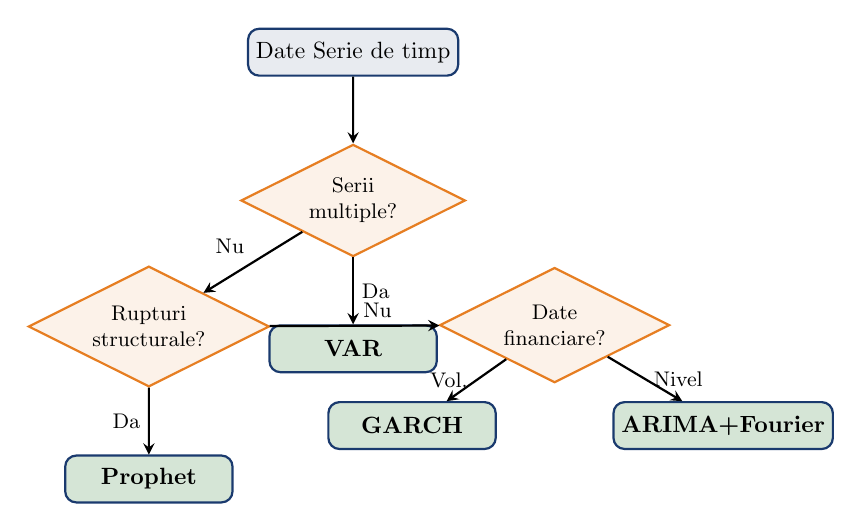
\begin{tikzpicture}[scale=0.85, transform shape,
        node distance=1.0cm,
        box/.style={rectangle, draw=MainBlue, thick, fill=MainBlue!10, rounded corners, minimum width=2.5cm, minimum height=0.7cm, align=center},
        decision/.style={diamond, draw=Orange, thick, fill=Orange!10, aspect=2, align=center, font=\small},
        arrow/.style={->, thick, >=stealth}
    ]
        \node[box] (start) {Date Serie de timp};
        \node[decision, below=of start] (q1) {Serii\\multiple?};
        \node[decision, below left=1.0cm and 1.3cm of q1] (q2) {Rupturi\\structurale?};
        \node[decision, below right=1.0cm and 1.3cm of q1] (q3) {Date\\financiare?};
        \node[box, fill=Forest!20, below=of q1] (var) {\textbf{VAR}};
        \node[box, fill=Forest!20, below=of q2] (prophet) {\textbf{Prophet}};
        \node[box, fill=Forest!20, below left=0.7cm and 0cm of q3] (garch) {\textbf{GARCH}};
        \node[box, fill=Forest!20, below right=0.7cm and 0cm of q3] (arima) {\textbf{ARIMA+Fourier}};
        \draw[arrow] (start) -- (q1);
        \draw[arrow] (q1) -- node[right] {\small Da} (var);
        \draw[arrow] (q1) -- node[above left] {\small Nu} (q2);
        \draw[arrow] (q2) -- node[left] {\small Da} (prophet);
        \draw[arrow] (q2) -- node[above right] {\small Nu} (q3);
        \draw[arrow] (q3) -- node[left] {\small Vol.} (garch);
        \draw[arrow] (q3) -- node[right] {\small Nivel} (arima);
    \end{tikzpicture}
    \end{center}
\end{frame}

\begin{frame}{Sumar: comparație modele}
    \begin{center}
        \includegraphics[width=0.95\textwidth, height=0.78\textheight, keepaspectratio]{../charts/model_comparison.pdf}
    \end{center}
    \quantlet{TSA\_ch10\_model\_comparison}{https://github.com/QuantLet/TSA/tree/main/TSA_ch10/TSA_ch10_model_comparison}
\end{frame}

\begin{frame}{Sinteză: Comparația modelelor}
    \begin{center}
    \footnotesize
    \begin{tabular}{lcccc}
        \toprule
        \textbf{Caracteristică} & \textbf{GARCH} & \textbf{Fourier} & \textbf{Prophet} & \textbf{VAR} \\
        \midrule
        \textbf{Țintă} & Volatilitate & Nivel & Nivel & Multiple \\
        \textbf{Sezonalitate} & Nu & Da (lungă) & Da (multiplă) & Nu \\
        \textbf{Rupturi structurale} & Nu & Nu & Da & Nu \\
        \textbf{Serii multiple} & Nu & Nu & Nu & Da \\
        \textbf{Interpretabil} & Mediu & Ridicat & Ridicat & Ridicat \\
        \textbf{Parametri} & Puțini & $2K$ & Auto & Mulți \\
        \textbf{Date lipsă} & Nu & Nu & Da & Nu \\
        \midrule
        \textbf{Ideal pentru} & Finanțe & Cicluri & Business & Macro \\
        \bottomrule
    \end{tabular}
    \end{center}

    \vspace{0.3cm}

    \begin{columns}[T]
        \column{0.5\textwidth}
        \begin{block}{Rezultatele noastre}
            \begin{itemize}
                \item GARCH: MAE=1,82 (volatilitate)
                \item Fourier: RMSE=31,10 (cicluri)
                \item SARIMA: RMSE=0,12 (rupturi)
                \item VAR: RMSE mediu=1,53 (multi)
            \end{itemize}
        \end{block}

        \column{0.5\textwidth}
        \begin{exampleblock}{Insight cheie}
            \begin{itemize}\setlength{\itemsep}{0pt}
                \item Fiecare model excelează în domeniul său
                \item Arta constă în alegerea modelului potrivit caracteristicilor datelor
            \end{itemize}
        \end{exampleblock}
    \end{columns}
\end{frame}

\begin{frame}{Bune practici pentru prognoza aplicată}
    \footnotesize
    \begin{columns}[T]
        \column{0.5\textwidth}
        \begin{block}{Metodologie}
            \begin{enumerate}\setlength{\itemsep}{0pt}
                \item \textbf{Explorați} datele temeinic
                \item \textbf{Testați} staționaritatea
                \item \textbf{Împărțiți} train/validation/test
                \item \textbf{Comparați} modele pe validare
                \item \textbf{Raportați} metrici pe test
            \end{enumerate}
        \end{block}

        \vspace{0.1cm}

        \begin{alertblock}{Greșeli frecvente}
            \begin{itemize}\setlength{\itemsep}{0pt}
                \item Privirea în datele de test
                \item Supraajustare pe setul de antrenament
                \item Ignorarea ipotezelor modelului
                \item Neraportarea incertitudinii
            \end{itemize}
        \end{alertblock}

        \column{0.5\textwidth}
        \begin{exampleblock}{Sfaturi practice}
            \begin{itemize}\setlength{\itemsep}{0pt}
                \item Începeți simplu (random walk, naiv)
                \item Adăugați complexitate doar dacă e necesar
                \item Vizualizați prognoze vs. valori reale
                \item Verificați reziduurile pentru tipare
                \item Raportați intervale de încredere
            \end{itemize}
        \end{exampleblock}

        \vspace{0.1cm}

        \begin{block}{Amintiți-vă}
            \begin{itemize}\setlength{\itemsep}{0pt}
                \item ``Toate modelele sunt greșite, dar unele sunt utile.'' \hfill --- George E. P. Box
            \end{itemize}
        \end{block}
    \end{columns}
\end{frame}

%=============================================================================
% CONCLUSION
%=============================================================================

\begin{frame}{Prognoză vs Cauzalitate vs Decizie}
    \begin{center}
    \footnotesize
    \begin{tabular}{lll}
        \toprule
        \textbf{Obiectiv} & \textbf{Model} & \textbf{Focalizare} \\
        \midrule
        Predicție pură & ARIMA / ML & Acuratețe out-of-sample \\
        Risc financiar & GARCH & Volatilitate, VaR \\
        Dinamici macro & VAR & Interacțiuni multivariate \\
        Relații structurale & SVAR / VECM & Identificare cauzală \\
        Regimuri & Markov Switching & Schimbări de regim \\
        \bottomrule
    \end{tabular}
    \end{center}

    \vspace{0.3cm}

    \begin{alertblock}{Mesaj cheie}
        \begin{itemize}\setlength{\itemsep}{0pt}
            \item Nu există model universal
            \item Există \textbf{potrivire între model și problemă}
        \end{itemize}
    \end{alertblock}
\end{frame}

\begin{frame}{Concluzii cheie}
    \begin{cminipage}{0.95\textwidth}
    \small
    \begin{enumerate}
        \item \textbf{Metodologie Riguroasă}
        \begin{itemize}
            \item Împărțirea train/validation/test previne supraajustarea
            \item Setul de test trebuie să rămână neatins până la evaluarea finală
        \end{itemize}

        \vspace{0.2cm}

        \item \textbf{Potriviți Modelul cu Datele}
        \begin{itemize}
            \item Volatilitate financiară $\succ$ GARCH
            \item Sezonalitate lungă $\succ$ Termeni Fourier
            \item Rupturi structurale $\succ$ Prophet
            \item Serii multiple $\succ$ VAR
        \end{itemize}

        \vspace{0.2cm}

        \item \textbf{Interpretați Rezultatele cu Grijă}
        \begin{itemize}
            \item Cauzalitate Granger $\neq$ cauzalitate adevărată
            \item Performanța out-of-sample contează cel mai mult
            \item Modelele mai simple funcționează adesea mai bine
        \end{itemize}
    \end{enumerate}
    \end{cminipage}
\end{frame}

%=============================================================================
\section{Utilizare IA}
%=============================================================================

\begin{frame}{Rolul AI în modelarea seriilor de timp}
    \begin{columns}[T]
        \column{0.5\textwidth}
        \begin{exampleblock}{AI poate}
            \begin{itemize}\setlength{\itemsep}{0pt}
                \item Genera cod pentru estimare și prognoză
                \item Selecta modele (AutoML, grid search)
                \item Combina prognoze (ensemble)
                \item Detecta anomalii și pattern-uri
            \end{itemize}
        \end{exampleblock}

        \column{0.5\textwidth}
        \begin{alertblock}{Dar nu poate}
            \begin{itemize}\setlength{\itemsep}{0pt}
                \item Înlocui validarea statistică
                \item Detecta automat \textbf{data leakage}
                \item Garanta interpretare economică corectă
                \item Verifica ipotezele modelului
            \end{itemize}
        \end{alertblock}
    \end{columns}

    \vspace{0.3cm}

    \begin{block}{Principiu}
        \begin{itemize}\setlength{\itemsep}{0pt}
            \item AI este \textbf{instrument}, nu autoritate
            \item Validarea statistică rămâne responsabilitatea cercetătorului
        \end{itemize}
    \end{block}
\end{frame}

\begin{frame}{Exercițiu AI: Gândire critică}
    \begin{cminipage}{0.95\textwidth}
    \vspace{-3mm}
    \begin{block}{\footnotesize Prompt de testat în ChatGPT / Claude / Copilot}
        {\footnotesize
        ``Descarcă de pe FRED vânzările lunare cu amănuntul din SUA (seria RSXFS) din 2010-01 până în 2024-12 (180 observații). Fă o analiză completă a seriei de timp: descompunere, teste de staționaritate, selecție model (compară ETS, SARIMA și Prophet), prognoză pe 12 luni, evaluare cu RMSE/MAE/MASE pe un split temporal 70/15/15. Vreau cod Python de calitate publicabilă.''
        }
    \end{block}
    \vspace{-2mm}
    {\footnotesize
    \textbf{Exercițiu}:
    \begin{enumerate}\setlength{\itemsep}{0pt}
        \item Rulați prompt-ul într-un LLM la alegere și analizați critic răspunsul.
        \item Urmează fluxul corect? (grafic $\to$ descompunere $\to$ test $\to$ model $\to$ diagnostic $\to$ prognoză)
        \item Compară mai multe modele (ETS, ARIMA, SARIMA) cu benchmark-uri adecvate?
        \item Împărțirea train/test este făcută corect? Există scurgeri de date (data leakage)?
        \item Discută limitările și ipotezele modelului ales?
    \end{enumerate}
    }
    \vspace{-2mm}
    \begin{alertblock}{}
        {\footnotesize \textbf{Atenție}: Codul generat de AI poate rula fără erori și arăta profesional. \textit{Asta nu înseamnă că e corect.}}
    \end{alertblock}
    \end{cminipage}
\end{frame}

%=============================================================================
% QUIZ
%=============================================================================
\section{Quiz}

\begin{frame}{Întrebarea 1}
    \begin{cminipage}{0.95\textwidth}
    \begin{alertblock}{Întrebare}
        \begin{itemize}\setlength{\itemsep}{0pt}
            \item Ce model alegeți pentru a prognoza volatilitatea randamentelor financiare?
        \end{itemize}
    \end{alertblock}

    \vspace{0.3cm}

    \begin{block}{Variante de răspuns}

        \textcolor{MainBlue}{\textbf{(A)}} ARIMA --- captează tendințe și autocorelații\\[3pt]

        \textcolor{MainBlue}{\textbf{(B)}} GARCH --- modelează varianța condiționată\\[3pt]

        \textcolor{MainBlue}{\textbf{(C)}} Prophet --- detectează puncte de schimbare\\[3pt]

        \textcolor{MainBlue}{\textbf{(D)}} VAR --- model multivariat pentru interdependențe

    \end{block}
    \end{cminipage}
\end{frame}

\begin{frame}{Întrebarea 1: Răspuns}
    \begin{cminipage}{0.95\textwidth}
    \vspace{-0.2cm}
    \begin{center}
        \includegraphics[width=0.98\textwidth, height=0.58\textheight, keepaspectratio]{ch10_quiz1_model_selection.pdf}
    \end{center}
    \vspace{-3mm}
    {\small
    \begin{exampleblock}{Răspuns: (B)}
    \begin{itemize}\setlength{\itemsep}{0pt}
        \item GARCH captează volatility clustering și riscul variabil în timp. ARIMA modelează nivelul, Prophet sezonalitatea, VAR relațiile între serii --- niciunul nu modelează varianța direct.
    \end{itemize}
    \end{exampleblock}
    }
    \hfill\quantlet{TSA\_ch10\_quiz1\_model\_selection}{https://github.com/QuantLet/TSA/tree/main/TSA_ch10/TSA_ch10_quiz1_model_selection}
    \end{cminipage}
\end{frame}

\begin{frame}{Întrebarea 2}
    \begin{cminipage}{0.95\textwidth}
    \begin{alertblock}{Întrebare}
        \begin{itemize}\setlength{\itemsep}{0pt}
            \item Un model SARIMA obține RMSE = 0,05 pe antrenament, dar RMSE = 2,30 pe test. Ce indică aceasta?
        \end{itemize}
    \end{alertblock}

    \vspace{0.3cm}

    \begin{block}{Variante de răspuns}

        \textcolor{MainBlue}{\textbf{(A)}} Modelul este excelent --- eroare mică pe antrenament\\[3pt]

        \textcolor{MainBlue}{\textbf{(B)}} Modelul suferă de overfitting --- memorează zgomotul\\[3pt]

        \textcolor{MainBlue}{\textbf{(C)}} Setul de test este greșit --- trebuie schimbat\\[3pt]

        \textcolor{MainBlue}{\textbf{(D)}} Diferența este normală --- nu e nicio problemă

    \end{block}
    \end{cminipage}
\end{frame}

\begin{frame}{Întrebarea 2: Răspuns}
    \begin{cminipage}{0.95\textwidth}
    \vspace{-0.2cm}
    \begin{center}
        \includegraphics[width=0.98\textwidth, height=0.58\textheight, keepaspectratio]{ch10_quiz2_overfitting.pdf}
    \end{center}
    \vspace{-3mm}
    {\small
    \begin{exampleblock}{Răspuns: (B)}
    \begin{itemize}\setlength{\itemsep}{0pt}
        \item Un raport de $46\times$ între RMSE test și train semnalează overfitting sever. Modelul se potrivește zgomotului din antrenament și nu generalizează. Soluție: model mai simplu, validare.
    \end{itemize}
    \end{exampleblock}
    }
    \hfill\quantlet{TSA\_ch10\_quiz2\_overfitting}{https://github.com/QuantLet/TSA/tree/main/TSA_ch10/TSA_ch10_quiz2_overfitting}
    \end{cminipage}
\end{frame}

\begin{frame}{Întrebarea 3}
    \begin{cminipage}{0.95\textwidth}
    \begin{alertblock}{Întrebare}
        \begin{itemize}\setlength{\itemsep}{0pt}
            \item De ce este importantă separarea datelor în train/validation/test?
        \end{itemize}
    \end{alertblock}

    \vspace{0.3cm}

    \begin{block}{Variante de răspuns}

        \textcolor{MainBlue}{\textbf{(A)}} Pentru a avea mai multe date de antrenament\\[3pt]

        \textcolor{MainBlue}{\textbf{(B)}} Pentru a preveni supraajustarea și a evalua corect\\[3pt]

        \textcolor{MainBlue}{\textbf{(C)}} Este doar o convenție, nu are importanță reală\\[3pt]

        \textcolor{MainBlue}{\textbf{(D)}} Pentru a reduce timpul de calcul

    \end{block}
    \end{cminipage}
\end{frame}

\begin{frame}{Întrebarea 3: Răspuns}
    \begin{cminipage}{0.95\textwidth}
    \vspace{-0.2cm}
    \begin{center}
        \includegraphics[width=0.98\textwidth, height=0.58\textheight, keepaspectratio]{ch10_quiz3_train_val_test.pdf}
    \end{center}
    \vspace{-3mm}
    {\small
    \begin{exampleblock}{Răspuns: (B)}
    \begin{itemize}\setlength{\itemsep}{0pt}
        \item Train: estimează parametrii. Validare: selectează modelul. Test: evaluare finală nebiasată. Amestecarea acestor roluri duce la estimări optimiste ale performanței.
    \end{itemize}
    \end{exampleblock}
    }
    \hfill\quantlet{TSA\_ch10\_quiz3\_train\_val\_test}{https://github.com/QuantLet/TSA/tree/main/TSA_ch10/TSA_ch10_quiz3_train_val_test}
    \end{cminipage}
\end{frame}

\begin{frame}{Întrebarea 4}
    \begin{cminipage}{0.95\textwidth}
    \begin{alertblock}{Întrebare}
        \begin{itemize}\setlength{\itemsep}{0pt}
            \item Cauzalitatea Granger este echivalentă cu cauzalitatea reală (structurală)?
        \end{itemize}
    \end{alertblock}

    \vspace{0.3cm}

    \begin{block}{Variante de răspuns}

        \textcolor{MainBlue}{\textbf{(A)}} Da --- dacă $X$ prezice $Y$, atunci $X$ cauzează $Y$\\[3pt]

        \textcolor{MainBlue}{\textbf{(B)}} Nu --- testează doar conținut predictiv, nu cauzalitate\\[3pt]

        \textcolor{MainBlue}{\textbf{(C)}} Depinde de numărul de lag-uri selectate\\[3pt]

        \textcolor{MainBlue}{\textbf{(D)}} Da, dacă p-value $< 0,05$

    \end{block}
    \end{cminipage}
\end{frame}

\begin{frame}{Întrebarea 4: Răspuns}
    \begin{cminipage}{0.95\textwidth}
    \vspace{-0.2cm}
    \begin{center}
        \includegraphics[width=0.98\textwidth, height=0.58\textheight, keepaspectratio]{ch10_quiz4_granger_causality.pdf}
    \end{center}
    \vspace{-3mm}
    {\small
    \begin{exampleblock}{Răspuns: (B)}
    \begin{itemize}\setlength{\itemsep}{0pt}
        \item Testul Granger verifică dacă trecutul lui $X$ îmbunătățește predicția lui $Y$. Corelații false (ex: vânzări de înghețată și înecuri) pot trece testul din cauza cauzelor comune.
    \end{itemize}
    \end{exampleblock}
    }
    \hfill\quantlet{TSA\_ch10\_quiz4\_granger\_causality}{https://github.com/QuantLet/TSA/tree/main/TSA_ch10/TSA_ch10_quiz4_granger_causality}
    \end{cminipage}
\end{frame}

\begin{frame}{Întrebarea 5}
    \begin{cminipage}{0.95\textwidth}
    \begin{alertblock}{Întrebare}
        \begin{itemize}\setlength{\itemsep}{0pt}
            \item Ce model folosiți pentru o serie cu sezonalitate lungă (ex: $s = 365$ zile)?
        \end{itemize}
    \end{alertblock}

    \vspace{0.3cm}

    \begin{block}{Variante de răspuns}

        \textcolor{MainBlue}{\textbf{(A)}} SARIMA$(p,d,q)(P,D,Q)_{365}$\\[3pt]

        \textcolor{MainBlue}{\textbf{(B)}} GARCH --- modelează variația\\[3pt]

        \textcolor{MainBlue}{\textbf{(C)}} ARIMA + Termeni Fourier sau Prophet/TBATS\\[3pt]

        \textcolor{MainBlue}{\textbf{(D)}} VAR cu 365 lag-uri

    \end{block}
    \end{cminipage}
\end{frame}

\begin{frame}{Întrebarea 5: Răspuns}
    \begin{cminipage}{0.95\textwidth}
    \vspace{-0.2cm}
    \begin{center}
        \includegraphics[width=0.98\textwidth, height=0.58\textheight, keepaspectratio]{ch10_quiz5_long_seasonality.pdf}
    \end{center}
    \vspace{-3mm}
    {\small
    \begin{exampleblock}{Răspuns: (C)}
    \begin{itemize}\setlength{\itemsep}{0pt}
        \item SARIMA$_{365}$ necesită $\sim$730 parametri sezonieri --- imposibil. Termenii Fourier cu $K=3$ folosesc doar 6 parametri. Prophet și TBATS gestionează sezonalități multiple automat.
    \end{itemize}
    \end{exampleblock}
    }
    \hfill\quantlet{TSA\_ch10\_quiz5\_long\_seasonality}{https://github.com/QuantLet/TSA/tree/main/TSA_ch10/TSA_ch10_quiz5_long_seasonality}
    \end{cminipage}
\end{frame}

%=============================================================================
% BIBLIOGRAFIE
%=============================================================================
\begin{frame}{Bibliografie I}
    \begin{block}{Manuale fundamentale (referințe comune tuturor capitolelor)}
        {\small
        \begin{itemize}
            \item Hamilton, J.D. (1994). \textit{Time Series Analysis}, Princeton University Press.
            \item Hyndman, R.J., \& Athanasopoulos, G. (2021). \textit{Forecasting: Principles and Practice}, 3rd ed., OTexts.
            \item Shumway, R.H., \& Stoffer, D.S. (2017). \textit{Time Series Analysis and Its Applications}, 4th ed., Springer.
        \end{itemize}
        }
    \end{block}

    \begin{exampleblock}{Lucrări de referință pe domenii}
        {\small
        \begin{itemize}
            \item Tsay, R.S. (2010). \textit{Analysis of Financial Time Series}, 3rd ed., Wiley. (GARCH, VAR)
            \item Lütkepohl, H. (2005). \textit{New Introduction to Multiple Time Series Analysis}, Springer. (VAR, VECM)
            \item Francq, C., \& Zakoïan, J.-M. (2019). \textit{GARCH Models}, 2nd ed., Wiley. (Volatilitate)
        \end{itemize}
        }
    \end{exampleblock}
\end{frame}

\begin{frame}{Bibliografie II}
    \begin{block}{Abordări moderne și competiții de prognoză}
        {\small
        \begin{itemize}
            \item Petropoulos, F., et al. (2022). Forecasting: Theory and Practice, \textit{International Journal of Forecasting}, 38(3), 845--1054.
            \item Makridakis, S., Spiliotis, E., \& Assimakopoulos, V. (2020). The M4 Competition, \textit{International Journal of Forecasting}, 36(1), 54--74.
            \item Taylor, S.J., \& Letham, B. (2018). Forecasting at Scale, \textit{The American Statistician}, 72(1), 37--45.
        \end{itemize}
        }
    \end{block}
\end{frame}

%=============================================================================
% SUMAR
%=============================================================================
\section{Sumar}

\begin{frame}{Concluzii esențiale}
\begin{block}{Ce am învățat}
\begin{itemize}
    \item Selectarea modelului depinde de caracteristicile datelor: staționaritate, sezonalitate, volatilitate
    \item Metodologia Box-Jenkins oferă un cadru sistematic pentru modelarea seriilor de timp
    \item Evaluarea corectă necesită testare out-of-sample și validare încrucișată
\end{itemize}
\end{block}

\begin{alertblock}{Important}
\begin{itemize}\setlength{\itemsep}{0pt}
    \item Niciun model nu câștigă peste tot --- potriviți modelul cu datele:
    \begin{itemize}\setlength{\itemsep}{0pt}
        \item ARIMA pentru tendințe
        \item SARIMA pentru sezonalitate
        \item GARCH pentru volatilitate
        \item VAR/VECM pentru dinamici multivariate
        \item Prophet/TBATS pentru tipare complexe
    \end{itemize}
    \item Validați întotdeauna out-of-sample!
\end{itemize}
\end{alertblock}
\end{frame}

%=============================================================================
% REFERINȚE
%=============================================================================
\begin{frame}{Referințe}
    \footnotesize
    \begin{thebibliography}{99}
        \bibitem{box2015} Box, G.E.P., Jenkins, G.M., Reinsel, G.C., \& Ljung, G.M. (2015). \textit{Time Series Analysis: Forecasting and Control}. 5th ed., Wiley.

        \bibitem{hamilton1994} Hamilton, J.D. (1994). \textit{Time Series Analysis}. Princeton University Press.

        \bibitem{tsay2010} Tsay, R.S. (2010). \textit{Analysis of Financial Time Series}. 3rd ed., Wiley.

        \bibitem{hyndman2021} Hyndman, R.J., \& Athanasopoulos, G. (2021). \textit{Forecasting: Principles and Practice}. 3rd ed., OTexts.

        \bibitem{taylor2018} Taylor, S.J., \& Letham, B. (2018). Forecasting at Scale. \textit{The American Statistician}, 72(1), 37-45.

        \bibitem{bollerslev1986} Bollerslev, T. (1986). Generalized Autoregressive Conditional Heteroskedasticity. \textit{Journal of Econometrics}, 31(3), 307-327.

        \bibitem{sims1980} Sims, C.A. (1980). Macroeconomics and Reality. \textit{Econometrica}, 48(1), 1-48.
    \end{thebibliography}
\end{frame}

\begin{frame}{}
    \centering
    \Huge\textcolor{MainBlue}{Vă Mulțumim!}

    \vspace{1cm}

    \Large Întrebări?

    \vspace{0.8cm}

    \normalsize

    Materialele cursului sunt disponibile la: \url{https://danpele.github.io/Time-Series-Analysis/}

    \vspace{0.2cm}

    \href{https://quantlet.com}{\raisebox{-0.15em}{\includegraphics[height=0.8em]{ql_logo.png}} Quantlet} \hspace{0.5cm}
    \href{https://quantinar.com}{\raisebox{-0.15em}{\includegraphics[height=0.8em]{qr_logo.png}} Quantinar}
\end{frame}

\end{document}
